\chapter{Computer vision}

\section{Le besoin}
L'utilisateur doit pouvoir rentrer la configuration de son cube dans le programme pour qu'il le résolve.
La façon la plus simple pour l'utilisateur de faire ça nous semblait être utiliser sa webcam.
Il aurait juste suffit à la personne de montrer son Rubik's à la webcam et le logiciel aurait "vu" les couleurs des différentes faces.

\section{Le choix de la bibliothèque}
L'idée au départ, était bien évidemment d'utiliser la bibliothèque \textit{OpenCV}, grande prêtresse dans le monde du traitement d'image.
Cependant, on s'est vite rendu compte que c'était un véritable calvaire d'intégrer ses packages nécessaire à son utilisation dans notre 
environnement de développement en Java. Des solutions existent comme le projet amateur JavaCV (cf . \url{https://github.com/bytedeco/javacv}).
Encore une fois, même si cela nous permettais d'avoir accès aux méthodes d'\textit{OpenCV}, il devient très délicat d'intégrer notre webcam
dans notre interface \textit{Swing} selon les versions utilisées d'\textit{OpenCV}. Après des recherches laborieuses durant plusieurs semaines 
sur internet, notre choix s'est porté sur la bibliothèque \textit{webcam-capture} (cf. \url{https://github.com/sarxos/webcam-capture}).

Malheureusement, celle bibliothèque ne propose aucune méthode d'analyse d'image, cette dernière est réalisée spécialement pour intégrer une webcam
sur une interface \textit{Swing} (quel aubaine !). Nous l'aurons donc, vous l'aurez compris, définir une méthode d'analyse de l'image.

\section{Analyse d'image}
Notre but est, je vous le rappelle, de pouvoir analyser les couleurs d'un Rubik's Cube afin de le résoudre. Plusieurs problèmes majeurs vont se poser à la capture.
Détaillons les ensemble afin de vous expliquer la façon choisie de s'en afranchir.
Partons du postulat qu'il est très facile de savoir la couleur d'un pixel sur une image.
En effet, il suffit d'appliquer la méthode \textit{getRGB} à une image de type \textit{BufferedImage}.
Supposons donc qu'il est facile de connaitre la couleur d'un pixel, faut-il encore s'assurer que le pixel en question est celui d'une face de notre Rubik's Cube.

Comme je vous l'ai dit, nous avons décidé de nous affranchir d'\textit{OpenCV}, il est donc impensable pour nous d'utiliser des méthodes de reconnaissance de contour
afin de connaitre la position sur l'image de notre facette. 
C'est pourquoi nous avons choisi d'imposer la position des facette à l'utilisateur en position, par dessus l'image sur l'interface (cf. l'image InteractivSolver\_capture
dans le chapitre 3), des points indiquant à l'utilisateur de placer les facettes par juxtaposition. De cette façon, qui est certe moins "user-friendly", nous avons simplement 
à analyser un nombre fixe de pixels. Encore mieux, ce sont toujours les même pixels qui seront analysés.

À partir d'ici, nous avons quasiment terminé. En effet, à une image donnée, on sait la position des facettes et il est possible de récupérer le code RGB de cette dernière. 
En pratique, nous prenont non pas 1 pixel, mais 25 (5*5) puis nous moyennons leur valeur pour s'éviter des valeurs abérantes.

Un nouveau problème est alors apparu : la dépendance du code RGB à l'environnement de capture. Le code RGB ne prenant pas en compte la luminosité ou la saturation, ses valeurs 
sont très fluctuante selon l'endroit où nous capturons notre Rubik's Cube. Il a alors fallu trouver un autre codage couleur : Le HSV.
Le HSV est l'accronyme de Hue, Saturation, Value of Brightness (parfois appelé HSB). Ce code, défini par trois nombres compris entre 0 et 1, permet de définir une couleur de façon 
beaucoup plus performante dans différents environnement. La valeur de H, qui définit la couleur en elle même, est beaucoup plus stable grâce aux valeurs de S et V. Il est alors beaucoup 
plus facile de définir des seuils empiriques pour choisir les couleurs.

Ce sont ces seuils qui ont été définis par la méthode \textit{defineColor} dans \textit{InteractivSolver\_capture}.
Ces seuils sont, comme je viens de le mentionner, définis empiriquement par échantillonnage (ci-dessous des valeurs moyennées de HSV des 6 couleurs faites à partir de 150 mesures par couleurs dans différents environnement).

\begin{figure}[H]
\begin{center}
	\makebox[\textwidth]{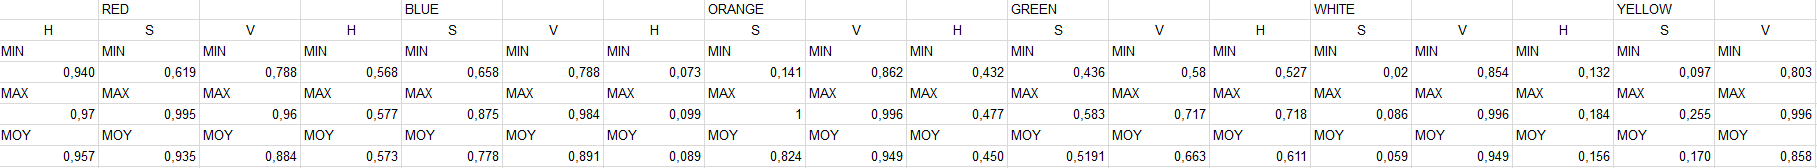
\includegraphics[width=.8\paperwidth]{diagrammes/Echantillonnage.png}}
\end{center}
	\caption{ \textit{Echantillonnage des valeurs HSV}}
\end{figure}

Ainsi, on peut remarquer que toutes les couleurs ont un domaine de H bien distinct mise à part la couleur blanche et bleu pour lesquelles il faut prendre la valeur de S qui sont bien différents entre les deux pour pouvoir les déterminer.

En pratique, ce système fonctionne dans la grande majorité des cas ce qui en fait un choix concluant pour la suite. Les analyses de couleurs fiables quelque soit la luminosité ambiante est un problème complexe qui fait l'objet de recherches
approfondies donc on peut s'estimer heureux d'avoir un système aussi fiable.

Maintenant, nous pouvons, à partir d'une image, analyser les facettes et connaître leur couleur. Nous venons donc d'élaborer un système de reconnaissance des couleurs.

Le dilemme maintenant est de s'assurer de la positions des différentes facettes que présente l'utilisateur pour éviter les configurations éronnées (comme un coin Blanc-Jaune-Blanc par exemple).
Nous demandons donc (cf. \textit{InteractivSolver\_capture} pour voir le code donnant les instructions) à l'utilisateur de poser face caméra le cube dans une position particulière (typiquement en fixant la face au dessus de celle présentée) de sorte 
à connaitre systématiquement les coordonnées des différentes facettes.

Nous y voilà, nous avons un système de Computer Vision qui est maintenant fonctionnel du Rubik's Cube, la grande difficulté restante étant la conversion de notre liste de couleurs que nous obtenons en une liste de permutations pour définir le Rubiks's Cube
et pourvoir le résoudre.






